
\begin{center}
\textit{\textbf{Corrigé officiel (éduscol)}}
\end{center}

\begin{enumerate}
\item Pour tout réel $x$, $f'(x) = (3 - 3x - 2)\e^x = (-3x + 1)\e^x$.

\item La fonction exponentielle étant strictement positive sur $\mathbb{R}$, le signe de $f'(x)$ est celui de $-3x + 1$.
\begin{center}
\begin{tikzpicture}
\tkzTabInit[lgt=2.5, espcl=3]{$x$ / 1, {Signe de $-3x + 1$} / 1, {Variations de $f$} / 2}{${-\infty}$, ${\frac13}$, ${+\infty}$}
\tkzTabLine{,+,0,-,}
\tkzTabVar{-/{$$},+/{$$},-/{$$}}{/}
\end{tikzpicture}
\end{center}
\end{enumerate}

\bigskip

